\section{Human Robot Interaction}

\begin{ejercicio}
    Explain the Sense-Think-Act paradigm in robotics. How does each component contribute to the overall autonomy of a robot, and what would happen if one component fails in a human-robot interaction scenario?

    The Sense-Think-Act paradigm is a fundamental framework in robotics that describes how robots perceive their environment, process information, and take actions based on that information. It has three main components:
    \begin{itemize}
        \item \textbf{Sense:} This component involves the robot's ability to gather data from its environment through sensors. It allows the robot to detect changes, obstacles, and other relevant information. Two main types of sensing are required:
        \begin{itemize}
            \item \ul{Internal Sensing:} This involves the robot's ability to monitor its own state, such as battery level, motor status, internal temperature and different internal sensors that provide feedback on the robot's health and functionality. For instance, if it has grippers, it can sense whether they are open or closed, and if it has wheels, it can sense their speed and direction.
            \item \ul{External Sensing:} This involves the robot's ability to perceive its surroundings, including objects, people, and environmental conditions. This can be achieved through various sensors such as cameras, LiDAR, ultrasonic sensors, and microphones. For example, a robot can use a camera to detect obstacles in its path or a microphone to recognize voice commands from humans.
        \end{itemize}
        \item \textbf{Think:} This component involves the robot's ability to process the sensed data and make decisions based on that information. It includes algorithms for perception, planning, and decision-making. An specific operating system is required, and a really typical example is ROS (Robot Operating System). Even though computers are usually pre-programmed and offline, a lot of research is being done to make them more autonomous and capable of learning from their environment (machine learning, deep learning, reinforcement learning, etc.) even in online scenarios.
        
        \item \textbf{Act:} This component involves the robot's ability to execute actions based on the decisions made in the Think phase. It includes actuators, motors, and other mechanisms that allow the robot to interact with its environment. For example, a robot can use its wheels to move towards a target location or its grippers to pick up an object.
    \end{itemize}

    If one component fails in a human-robot interaction scenario, it can significantly impact the robot's autonomy and effectiveness, as it would result in the robot being unable to perceive its environment, make informed decisions, or take appropriate actions. For example, if the Sense component fails, the robot may not be able to detect obstacles or recognize human commands, leading to potential accidents or misunderstandings.
\end{ejercicio}

\begin{ejercicio}
    Please read through the scenario and discuss whether the interactive system is a robot or not according to the Sense-Think-Act definition.
    \begin{itemize}
        \item A smart speaker that can play music, answer questions, and control smart home devices.
        
        According to the Sense-Think-Act definition, a smart speaker can be considered a robot. It has the ability to sense its environment through microphones and other sensors, think by processing the input data and making decisions based on that information, and act by executing commands such as playing music or controlling smart home devices. However, it is important to note that while a smart speaker strictly meets the criteria of the Sense-Think-Act paradigm, it may not have the physical embodiment or mobility typically associated with traditional robots.

        \item A robotic vacuum cleaner that can navigate a home, avoid obstacles, and clean floors.
        
        A robotic vacuum cleaner can also be considered a robot according to the Sense-Think-Act definition. It senses its environment using sensors such as cameras, LiDAR, or infrared sensors to detect obstacles and navigate the home. It thinks by processing the sensed data and making decisions on how to move and clean effectively. Finally, it acts by using its motors and brushes to clean the floors.
    \end{itemize}
\end{ejercicio}

\begin{ejercicio}
    What is the difference between coexistence, cooperation, and collaboration in HRI (according to Schmidtler et al., 2015)? Give one example task for each.

    This clasification refers to the different levels of interaction between humans and robots in a shared environment. All of them refer to tasks where the time and the space between the human and the robot is shared, but the level of interaction is different. The three levels are:
    \begin{itemize}
        \item \textbf{Coexistence:} In this level, humans and robots share the same environment at the same time, but they do not directly interact or influence each other's actions. An example task for coexistence could be a robot vacuum cleaner operating in a home while humans are present, but the humans do not interact with the robot or affect its cleaning path.
        \item \textbf{Cooperation:} In this level, humans and robots work together towards a common goal, but they do not necessarily have to coordinate their actions closely. An example task for cooperation could be a vacuum robot cleaning the floor while a human is cleanng the windows. Both are working towards the common goal of cleaning the house, but they do not need to coordinate their actions closely.
        \item \textbf{Collaboration:} In this level, humans and robots work closely together, coordinating their actions and sharing information to achieve a common goal. An example task for collaboration could be a human and a robot assembling furniture together, where the human holds pieces in place while the robot tightens screws or performs other assembly tasks, requiring close coordination and communication between the two.
    \end{itemize}
\end{ejercicio}

\begin{ejercicio}
    Explain the difference between the ``inside-out'' and ``outside-in'' approaches in HRI. In the following scenario, which approach would you choose and why?
    \begin{enumerate}
        \item You are designing a robot to assist elderly people in their daily activities, such as reminding them to take their medication, helping them with mobility, and providing companionship. The robot should be able to adapt to the individual needs and preferences of each elderly person.
    \end{enumerate}

    Both approaches refer to different ways of designing and implementing human-robot interaction systems. The ``inside-out'' approach firstly focuses on developping the technology and capabilities of the robot, and then adapts the human interaction to fit the robot's capabilities. In contrast, the ``outside-in'' approach starts by understanding the human user's needs, preferences, and behaviors, and then designs the robot's capabilities and interaction methods to align with those human factors.
    \begin{enumerate}
        \item In the scenario of designing a robot to assist elderly people, I would choose the ``outside-in'' approach. This is because the primary goal is to meet the individual needs and preferences of each elderly person, which requires a deep understanding of their daily routines, challenges, and expectations. By starting with the human user's perspective, we can ensure that the robot's capabilities and interaction methods are tailored to provide meaningful assistance and companionship. This approach would likely lead to higher user satisfaction, better adoption rates, and more effective support for the elderly individuals.
    \end{enumerate}
\end{ejercicio}

\begin{ejercicio}
    Given the two graphical representations in Figure~\ref{fig:uncanny_valley_ej}, explain which one represents the ``Uncaney Valley'' effect and why. What do you have to consider when designing a robot to avoid this effect?

    \begin{figure}
        \centering
        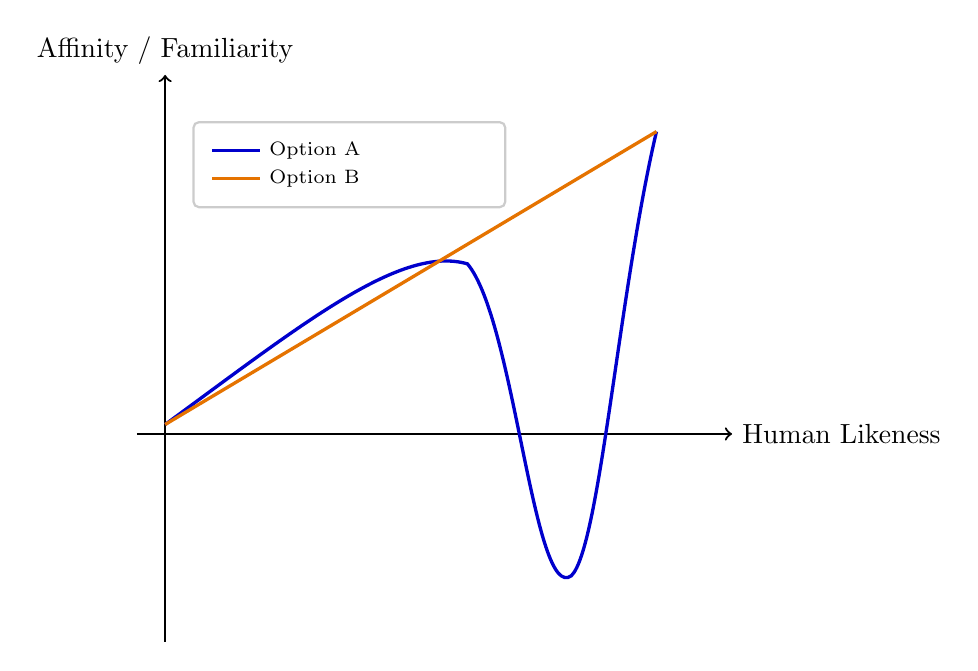
\begin{tikzpicture}[scale=1.2]

            % Grid axes
            \draw[->, thick] (-0.3,0) -- (6.0,0) node[right] {Human Likeness};
            \draw[->, thick] (0,-2.2) -- (0,3.8) node[above] {Affinity / Familiarity};

            % --------------------------------------------------
            % GRAPH A: Uncanny Valley Curve (Actual Model - Blue)
            % --------------------------------------------------
            \draw[very thick, blue!80!black] 
                (0,0.1) 
                .. controls (1.5,1.2) and (2.5,2.0) .. (3.2,1.8) 
                .. controls (3.7,1.2) and (3.9,-1.8) .. (4.3,-1.5) 
                .. controls (4.6,-1.2) and (4.8,1.5) .. (5.2,3.2);

            % --------------------------------------------------
            % GRAPH B: Linear Hypothesis (Hypothetical / False - Orange)
            % --------------------------------------------------
            \draw[very thick, orange!90!black] (0,0.1) -- (5.2,3.2);

            % Legend Box
            \begin{scope}[shift={(0.3,2.4)}]
                \draw[thick, fill=white, draw=gray!40, rounded corners=2pt] (0,0) rectangle (3.3,0.9);
                \draw[very thick, blue!80!black] (0.2,0.6) -- (0.7,0.6);
                \node[right, font=\scriptsize] at (0.7,0.6) {Option A};
                \draw[very thick, orange!90!black] (0.2,0.3) -- (0.7,0.3);
                \node[right, font=\scriptsize] at (0.7,0.3) {Option B};
            \end{scope}

        \end{tikzpicture}
        \caption{Comparison between the actual Uncanny Valley curve and a hypothetical model.}
        \label{fig:uncanny_valley_ej}
    \end{figure}

    In Figure~\ref{fig:uncanny_valley_ej}, the blue curve (Option A) represents the ``Uncanny Valley'' effect. This effect describes a phenomenon where as a robot's appearance becomes more human-like, people tend to feel more affinity and familiarity towards it, up to a certain point. However, when the robot's appearance is very close to human but not quite perfect, it can evoke feelings of eeriness or discomfort, leading to a sharp drop in affinity. This is represented by the dip in the blue curve.

    In order to avoid the Uncanny Valley effect when designing a robot, if the designer aims for a android and human-like appearance, it is important to ensure that the robot's features are either clearly non-human or highly realistic and indistinguishable from a real human. Designers should focus on achieving a balance between human-like characteristics and maintaining a level of abstraction that prevents the robot from appearing unsettling.
\end{ejercicio}

\begin{ejercicio}
    Why is robot design usually a ``wicked'' problem?

    A wicked problem is a complex issue that is difficult to define and has no clear nor definitive solution. In the context of robot design, it is considered a wicked problem because it involves multiple stakeholders with different perspectives, values, and goals. Additionally, the design process is iterative and may require continuous adjustments based on user feedback and changing requirements.
\end{ejercicio}


\begin{ejercicio}
    In order for humans to really collaborate with robots, the robots have to communicate their intents to the humans. Describe two ways in which a robot could communicate the intent to give an object to a human and discuss the pros and cons.
    \begin{itemize}
        \item \textbf{Verbal Communication:} The robot could use speech to inform the human that it intends to give them an object. For example, it could say, ``Please, I am handing you the object now.'' It has the advantage of being clear and direct, allowing the human to understand the robot's intent easily. However, it may not be effective in noisy environments or for individuals with hearing impairments.
        \item \textbf{Nonverbal Communication:} The robot could use gestures or body language to indicate its intent. For example, it could extend its arm towards the human while holding the object and still respecting the social zones. This method can be more intuitive and can be understood even in noisy environments. However, it may be less precise than verbal communication and could lead to misunderstandings if the gestures are not clear or culturally appropriate.
    \end{itemize}
\end{ejercicio}

\begin{ejercicio}
    Compare verbal and nonverbal interaction in HRI. Give two examples of nonverbal interaction methods.

    Verbal interaction in HRI involves the use of spoken language to communicate between humans and robots, while nonverbal interaction encompasses all forms of communication that do not rely on words, such as gestures, facial expressions, body language, and other visual or auditory cues. Both forms of interaction are important for effective communication and collaboration between humans and robots, as they can complement each other and provide additional context or clarity. Some examples of nonverbal interaction methods include:
    \begin{itemize}
        \item \textbf{Gestures:} Robots can use hand movements, arm gestures, or other body movements to convey information or intentions. For example, a robot could wave to greet a human or point to an object to indicate that it wants the human to pick it up.
        \item \textbf{Gaze and Eye Contact:} Robots can use their eyes or head movements to establish eye contact with humans, which can help convey attention, interest, or engagement. For example, a robot could look directly at a human when asking a question or when waiting for a response, signaling that it is actively listening and engaged in the interaction.
    \end{itemize}
\end{ejercicio}

\begin{ejercicio}
    Why shouldn't we neglect nonverbal communication when designing a robot? Provide 2 reasons and examples for them.

    Nonverbal communication is a crucial aspect of human-robot interaction (HRI) that should not be neglected in robot design for several reasons:
    \begin{itemize}
        \item \textbf{Noise and Environmental Factors:} In many real-world scenarios, verbal communication may be hindered by background noise or other environmental factors. Nonverbal cues, such as gestures, facial expressions, or body language, can provide additional context and help convey information even when verbal communication is not possible. For example, a robot could use hand gestures to indicate directions or point to an object in a noisy factory setting where verbal instructions may not be heard clearly.
        \item \textbf{Hearing Impairments and Accessibility:} Some individuals may have hearing impairments or other conditions that make verbal communication challenging. Nonverbal communication methods can help ensure that these individuals can still effectively interact with robots. For example, a robot could use visual cues, such as flashing lights or on-screen text, to convey important information to users who may not be able to hear spoken instructions.
        \item \textbf{Cultural Differences:} Even though the language spoken in each country is different, the nonverbal communication (although it is also culturally dependent) is more universal. For example, a robot could use a thumbs-up gesture to indicate approval or agreement, which is generally understood across many cultures, even if the verbal language used by the robot is not.
    \end{itemize}
\end{ejercicio}

\begin{ejercicio}
    A robot is deployed in a classroom to invigilate students writing exams. How could the robot look? Give reasons for your answer.

    Since the students are more used to seeing humans in the classroom, the robot should have a humanoid appearance and be antropomorphic. This would make the students feel more comfortable and less intimidated by the robot's presence. In order to avoid the Uncanny Valley effect, and given that achieving a perfect human-like appearance is very difficult, the robot should not be too realistic. Instead, it should have a simplified and stylized humanoid design that is clearly robotic but still relatable to humans.

    Regarding the robot's height, it should be similar to that of a human adult, so that it resembles a teacher or invigilator. In order to be able to monitor the whole class from above, it should have a head with eyes that can move around, and a camera that records in the direction of the students. Since binoccularity vision is not needed, the robot could have a single camera in the middle of its head. Regarding the movements, it should have wheels to move around the classroom. Since rotating the head can be disconcerting and uncomfortable for the students, the robot should only be allowed to tilt the head, but not rotate it. Instead, it should rotate the whole body using the wheels to change the direction of the head. The wheels should be high enough and with a robust motor to be able to move around the classroom without any problems. It should also include LiDAR sensors to detect obstacles and avoid collisions with students or furniture.

    In order to avoid the robot being too intimidating, and given that it is not necessary for the robot to have arms, it should not have them in order to meet the affordance of the robot. However, as it would have a microphone (to hear the students cheating) and a speaker (to give instructions to the students), it should have ears and a mouth, but they should be stylized and simplified to avoid the Uncanny Valley effect.
\end{ejercicio}

\begin{ejercicio}
    For a holiday job, students need to be taught how to correctly place goods in a supermarket. Instead of a human assistant, you want to use a robot to demonstrate and explain the tasks that need to be completed, as well as to check whether the trainee is missing any steps. What kind of robot would you use in this setting?\\

    In this setting, since students want to directly learn from the robot, it should have a humanoid appearance and be antropomorphic, as they want to repeat the same actions as the robot. In order to avoid the Uncanny Valley effect, and given that achieving a perfect human-like appearance is very difficult, the robot should not be too realistic. Instead, it should have a simplified and stylized humanoid design that is clearly robotic but still relatable to humans.

    As the robot needs to demonstrate and explain the tasks, it should have arms and hands to be able to manipulate the goods and show the correct placement, legs and knees to be able to grab the goods from the floor with a correct back posture, and a head with eyes to be able to look at the goods and the students and a mouth to be able to explain the tasks. Since it would also hear the students asking questions, it should have ears. A microphone, speaker and a camera should be included in the head to be able to hear, speak and see the students.

    Regaring the movements, it should use the legs to move around the supermarket, so no wheels are needed. The arms should have a good range of motion to be able to reach the goods and demonstrate the correct placement. The hands should have a good grip to be able to hold the goods securely.
\end{ejercicio}

\begin{ejercicio}
    How does the concept of ``affordance'' influence children's perception of educational robots, and how should it be considered in the design of such robots (e.g., telepresence robots for remote learners)?

    The concept of ``affordance'' refers to the perceived and actual properties of an object that determine how it can be used. A robot should always underpromise its capabilities and functionalities (so that the user does not expect more than what the robot can do) and overdeliver (so that the user is positively surprised by the robot's capabilities). In addition, the form of a robot should be designed to suggest its intended use and functionality, making it intuitive for children to understand how to interact with the robot. If children see a robot with grippers, they will expect it to be able to pick up objects, and if they see a robot with a screen, they will expect it to be able to display information. Therefore, the design of educational robots should consider the affordances that are relevant to the intended educational tasks and interactions, ensuring that children can easily understand how to use the robot effectively.
\end{ejercicio}

\begin{ejercicio}
    You are designing a robot to assist elderly people at home. Using the concepts of affordance, anthropomorphism, and social zones, outline key design considerations.

    Regarding affordance, the robot should have clear and intuitive features that suggest its intended use. It should have grippers to catch objects and hand them to the elderly person and a screen to display information, for instance. However, in order to have an intuitive and easy-to-use interface, the robot should not have too many buttons or complex controls, only voice commands.

    Regarding anthropomorphism, the robot should have a humanoid appearance and be antropomorphic, as it would make the elderly person feel more comfortable and less intimidated by the robot's presence. Since they are not used to seeing robots, it should have a simplified and stylized humanoid design that is clearly robotic (to avoid the Uncanny Valley effect) but still relatable to humans.

    Regarding social zones, the robot should respect the personal space of the elderly person and maintain an appropriate distance during interactions. However, as the elderly person may have mobility issues, the robot should be able to approach them when necessary, such as when handing them an object or providing assistance when standing up (if needed). In addition, as the percieved security is not the same as the real security, the robot should always move using a slow and smooth motion, and it should never approach the elderly person from behind, as it could startle them.
\end{ejercicio}

\begin{ejercicio}
    You want to develop a robot that can help kids in school to learn about mathematics. Which morphological structure would you use to make the robot the best option for working with kids and why?

    When designing a robot to help kids learn mathematics, I would choose a humanoid morphological structure. This is because children are more likely to relate to and engage with a robot that has human-like features, making the learning experience more interactive and enjoyable. A humanoid robot can use gestures, facial expressions, and body language to communicate concepts effectively, which can enhance understanding and retention of mathematical concepts.
\end{ejercicio}

\begin{ejercicio}
    Given the robots in Figure~\ref{fig:robot_options}, which one would you choose for the following scenarios and why?
    \begin{figure}
        \centering
        \begin{subfigure}[b]{0.2\textwidth}
            \centering
            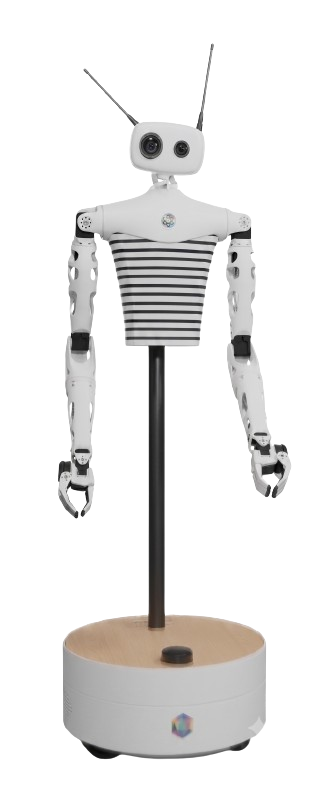
\includegraphics[width=\textwidth]{img/robots/robot1.png}
            \caption{Option A}
            \label{subfig:robot_a}
        \end{subfigure}
        \hspace{0.05\textwidth}
        \begin{subfigure}[b]{0.2\textwidth}
            \centering
            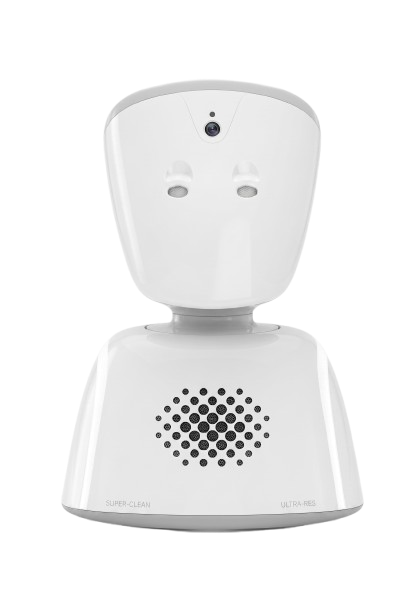
\includegraphics[width=\textwidth]{img/robots/robot2.png}
            \caption{Option B}
            \label{subfig:robot_b}
        \end{subfigure}
        \hspace{0.05\textwidth}
        \begin{subfigure}[b]{0.2\textwidth}
            \centering
            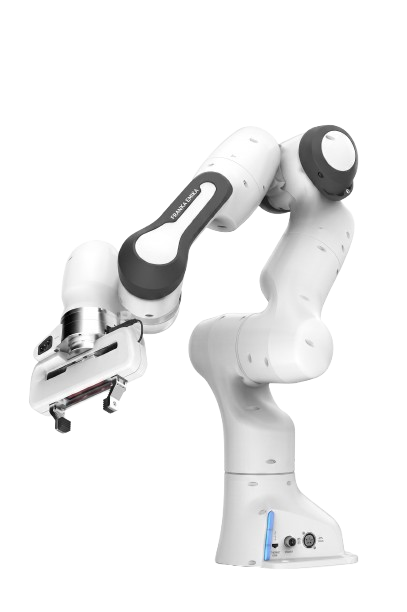
\includegraphics[width=\textwidth]{img/robots/robot3.png}
            \caption{Option C}
            \label{subfig:robot_c}
        \end{subfigure}
        \hspace{0.05\textwidth}
        \begin{subfigure}[b]{0.2\textwidth}
            \centering
            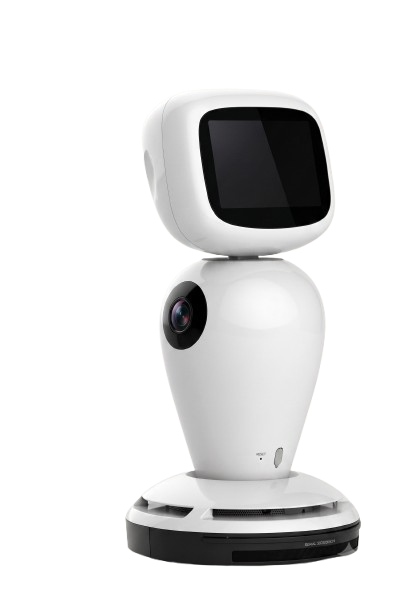
\includegraphics[width=\textwidth]{img/robots/robot4.png}
            \caption{Option D}
            \label{subfig:robot_d}
        \end{subfigure}

        \caption{Comparison of the four robot models.}
        \label{fig:robot_options}
    \end{figure}
    \begin{itemize}
        \item The robot is supposed to be an avatar for children in class who are currently hospitalized and cannot attend class.
        
        In this case, I would choose Option~\ref{subfig:robot_d}. Since the student should ideally be able to move around the class to speak with the teacher and classmates, Option~\ref{subfig:robot_b} and Option~\ref{subfig:robot_c} are not suitable, as they are not mobile. Option~\ref{subfig:robot_a} is mobile, but it has grippers, which are not needed in this scenario and could be dangerous for the children. In addition, regarding affordance, if the robot had grippers the other students could think that the robot can pick up objects, which is not the case. Therefore, Option~\ref{subfig:robot_d} is the best option.

        Since the student would be able to move and speak, eyes and a mouth should be displayed in the screen, so that the other students can see the student's face and expressions.
    \end{itemize}
\end{ejercicio}